\chapter{Lösung des Problems}

Entgegen der Intuition der Meisten, besagt die Lösung des Ziegenproblems von vos Savos, man hätte eine Gewinnchance von \sfrac{2}{3} wenn man wechselt, während man bei der ursprünglichen Wahl nur in \sfrac{1}{3} der Fälle das Auto gewinnt:

\begin{quote}
    Ja; Sie sollten wechseln. Das erste Tor hat eine Chance von \sfrac{1}{3} zu gewinnen, aber das Zweite hat eine \sfrac{2}{3} Chance. Hier ist eine gute Möglichkeit um darzustellen was passiert ist. Angenommen es gäbe eine millionen Tore, und Sie wählen Tor 1. Dann öffnet der Host, der weiß was hinter jedem Tor ist und immer das Tor mit dem Gewinn vermeidet, alle Tore außer das Tor mit der Nummer 777777. Sie würden direkt wechseln, oder? (\cite{Savant:1990})
\end{quote}

Anders erklärt, kann man auch folgendermaßen argumentieren: Dass der Kandidat auf Anhieb das richte Tor erwischt liegt bei der A-priori-Wahrscheinlichkeit von \sfrac{1}{3} und dass das Auto hinter einem der anderen Tore steht bei \sfrac{2}{3}. Wird nun ein Tor geöffnet, kann sich die Wahrscheinlichkeit, dass die erste Wahl richtig war nicht geändert haben. Dadurch liegen die Wahrscheinlickeiten der übrigen Tore nicht bei \sfrac{1}{2}. Vielmehr steht hinter dem Tor, das nicht zuerst gewählt war und nicht vom Moderator geöffnet wurde, mit einer Wahrscheinlichkeit von \sfrac{2}{3} das Auto.

\begin{figure}[htbp]
    \centering
    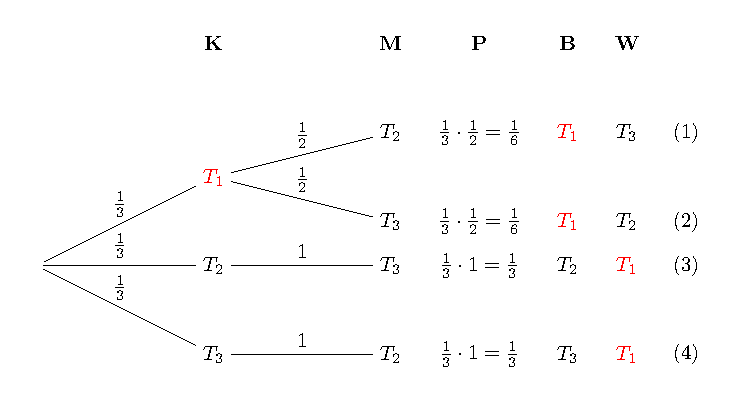
\includegraphics{tex/tree.pdf}
    \caption{Entscheidungsbaum}\label{fig:tree}
    \small {Der Baum stellt den Ablauf der Spieleshow für den Fall, dass hinter dem ersten Tor ($T_1$) das Auto steht, dar. Zunächst trifft der Kandidat seine erste Wahl (K). Anschließend öffnet der Moderator ein Ziegentor, dass nicht vom Kandidaten gewählt wurde (M). Entlag der Pfade werden die Wahrscheinlicketen mutipliziert (P). (B) und (W) zeigen die Tore, die man beim Bleiben bzw. beim Wechseln öffnen würde.}
\end{figure}

Der Entscheidungsbaum in \autoref{fig:tree} veranschaulicht alle Fälle, bei denen das Auto hinter dem ersten Tor steht. Bei den Fällen (1) und (2) gewinnt man, wenn man nicht wechselt, mit Wechseln gewinnt man in den Fällen (3) und (4). Addiert man die Wahrscheinlichkeiten der jeweiligen Pfade erhällt man die Gewinnwahrscheinlichkeiten das Auto zu gewinnen beim Bleiben $P_B(Auto)$ und Wechseln $P_W(Auto)$:

\begin{align*}
    P_B(Auto) & = P(T_1T_2) + P(T_1T_3)                   \\
              & = \frac{1}{6} + \frac{1}{6} = \frac{1}{3} \\
    P_W(Auto) & = P(T_2T_3) + P(T_3T_2)                   \\
              & = \frac{1}{3} + \frac{1}{3} = \frac{2}{3} \\
\end{align*}

Somit haben wir die Lösung von vos Savos bestätigt.


